\chapter{Nearest neighbors: local prediction, retrieval, and engineering}
\label{ch:nearest-neighbors}

\begin{learningobjectives}
After this chapter, you should be able to:
\begin{itemize}
  \item define nearest-neighbor classification and regression from a metric,
  neighborhood, weighting rule, and aggregation rule;
  \item explain how representation, scaling, dimension, and $k$ determine a
  local model's statistical behavior;
  \item construct an item-item collaborative-filtering recommender and state
  what its offline evidence can and cannot establish;
  \item implement nearest-neighbor estimators as typed, tested package code
  rather than notebook-only functions; and
  \item place data, fixtures, algorithms, tests, experiments, and operational
  evidence in defensible repository boundaries.
\end{itemize}
\end{learningobjectives}

\begin{chapterconnection}
The preceding chapters learned affine scores, margins, compositions, and dense
representations. Nearest neighbors takes a different position: retain the
training observations and answer a query from nearby evidence. The fitted
object has few numerical coefficients, but it has strong assumptions. A
representation defines which differences are visible; a metric defines
closeness; $k$ defines locality; an aggregation rule turns neighbors into an
answer; and a system must store and search the resulting evidence under latency,
memory, privacy, and update constraints.
\end{chapterconnection}

\section{A local principle with a long history}

Nearest-neighbor methods formalize a simple proposition: observations that are
near one another in a defensible representation should have related responses.
Fix and Hodges studied nearest-neighbor discrimination in 1951. Cover and Hart's
1967 analysis made the one-nearest-neighbor rule a foundational result in
statistical pattern recognition. The method remains useful because it is both a
model and a diagnostic. It supplies a transparent nonlinear baseline, exposes
whether a representation creates coherent neighborhoods, and provides the
retrieval operation beneath recommendation, similarity search, and some anomaly
systems.

Calling kNN \emph{nonparametric} does not mean that it has no choices, performs
no fitting, or automatically ignores irrelevant variables. It means that the
model is not confined to a fixed finite-dimensional parameter vector as the
sample grows. Training observations themselves are fitted state. The method has
hyperparameters---metric, $k$, weights, preprocessing, search strategy---and its
effective complexity can grow with the data.

\begin{misconceptionbox}
\textbf{Misconception:} nonparametric methods accept every available feature and
ignore useless ones. \textbf{Correction:} every included coordinate can change
distance and therefore neighbor identity. Independent noise dimensions may
overwhelm useful local structure. Representation selection is part of the model.
\end{misconceptionbox}

\section{The mathematical object: a neighborhood}

Let
\[
D=\{(x_i,y_i)\}_{i=1}^{n},\qquad x_i\in\mathcal X,
\]
be a supervised training set. The response $y_i$ is numerical for regression
and belongs to a finite class set $\mathcal C$ for classification. A metric
$d:\mathcal X\times\mathcal X\to[0,\infty)$ satisfies
\begin{align*}
d(x,z)&\ge 0, & d(x,z)=0&\Longleftrightarrow x=z,\\
d(x,z)&=d(z,x), & d(x,z)&\le d(x,u)+d(u,z).
\end{align*}
For a query $x$, write $N_k(x)$ for the indices of the $k$ training
observations with smallest $d(x,x_i)$. A complete implementation also declares
how exact distance ties are ordered.

For vectors in $\mathbb R^p$, the Minkowski family is
\[
d_q(x,z)=\left(\sum_{j=1}^{p}|x_j-z_j|^q\right)^{1/q},\qquad q\ge 1.
\]
$q=1$ is Manhattan distance and $q=2$ is Euclidean distance. Other domains need
other structures: angular similarity for direction, Hamming distance for binary
attributes, geodesic distance on a sphere, edit distance for sequences, or a
domain-specific combination of continuous and categorical differences. A
formula is not defensible merely because software provides it.

\conceptcheck{Suppose a dataset records temperature in degrees Celsius and
annual income in dollars. Which coordinate is likely to dominate raw Euclidean
distance? Why does standardization address numerical scale without proving that
one standard deviation has equal scientific meaning in both variables?}

\subsection{Classification by local vote}

Uniform kNN estimates a class probability by a local frequency:
\[
\widehat P_k(Y=c\mid X=x)
=\frac{1}{k}\sum_{i\in N_k(x)}\mathbf 1\{y_i=c\},
\]
and predicts
\[
\widehat g_k(x)=\arg\max_{c\in\mathcal C}
\widehat P_k(Y=c\mid X=x).
\]
The vote vector sums to one, but it is not automatically a calibrated
probability vector. The neighborhood is data-dependent, classes may be
imbalanced, and $k$ may have been selected for a metric other than calibration.
A deterministic class-tie policy belongs in the public contract.

\subsection{Regression by local averaging}

Uniform kNN regression estimates a local conditional mean:
\[
\widehat f_k(x)=\frac{1}{k}\sum_{i\in N_k(x)}y_i.
\]
It is piecewise constant under a fixed training set. It interpolates local
evidence rather than extending a global trend, so it can behave poorly outside
training support even though it always returns a number.

\subsection{Distance-weighted aggregation}

A weighted rule replaces equal contributions with nonnegative weights:
\[
\widehat f(x)=
\frac{\sum_{i\in N_k(x)}w_i(x)y_i}
{\sum_{i\in N_k(x)}w_i(x)},
\qquad w_i(x)=\frac{1}{d(x,x_i)}.
\]
Classification replaces $y_i$ with class indicators. Exact matches require an
explicit zero-distance policy. A common contract assigns vote mass only to exact
matches, preventing division by zero and preventing distant observations from
diluting identical inputs. Conflicting labels at identical inputs should also
trigger a data-quality investigation.

\begin{figure}[htbp]
  \centering
  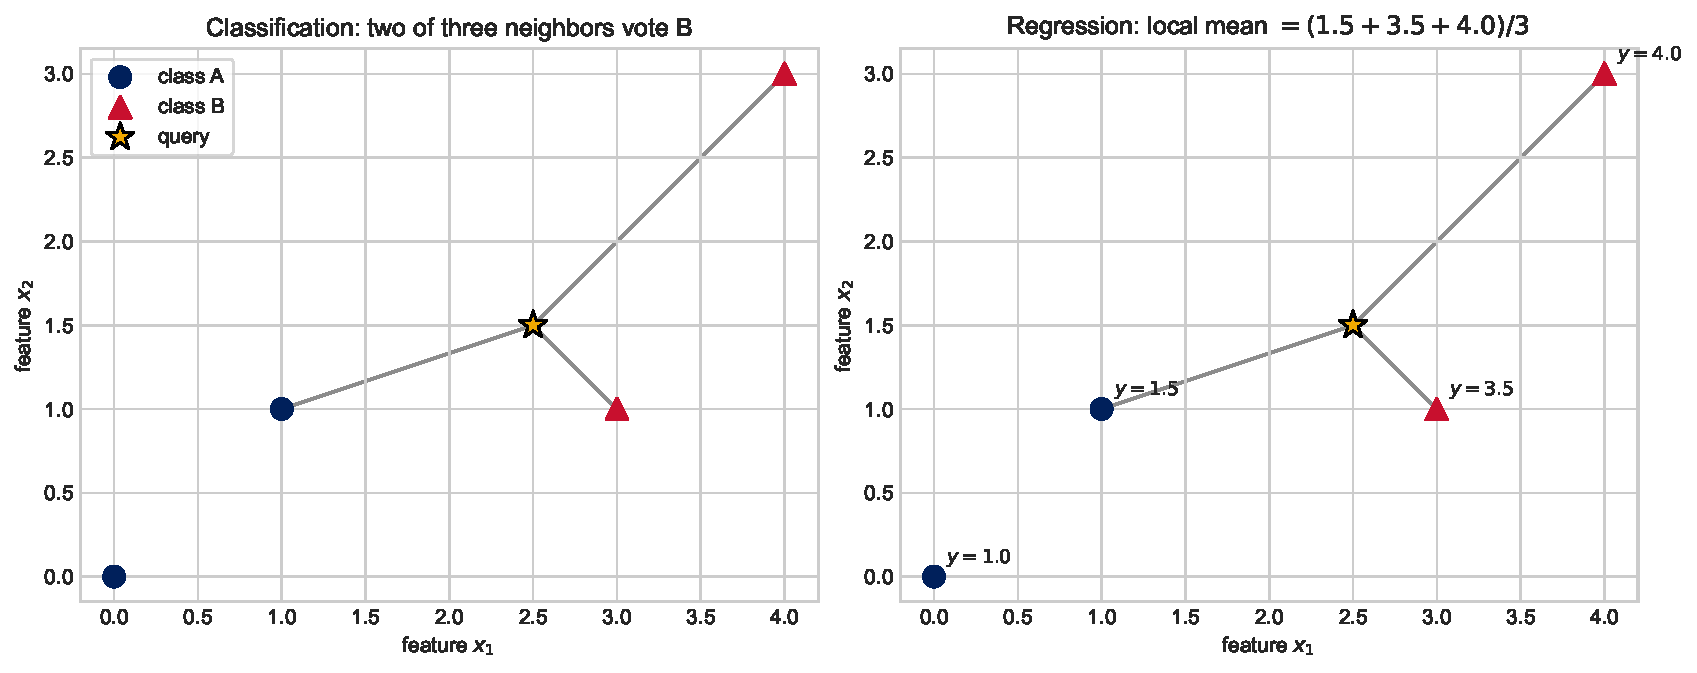
\includegraphics[width=0.98\textwidth]{figures/generated/knn-local-aggregation.pdf}
  \caption{The neighbor search is shared, while the target contract determines
  aggregation. Classification votes over labels; regression averages numerical
  responses. The query's three selected neighbors are drawn explicitly.}
  \label{fig:knn-local-aggregation}
\end{figure}

\begin{workedexample}{one search, two prediction tasks}
Let training features be
\[
(0,0),\ (1,1),\ (3,1),\ (4,3)
\]
and let the query be $x=(2.5,1.5)$. The Euclidean distances are approximately
$2.92$, $1.58$, $0.71$, and $2.12$. Thus the three-neighbor index set contains
rows $3$, $2$, and $4$ when rows are numbered from one.

If their class labels are B, A, and B, then the class vote is two-thirds B. If
their numerical responses are $3.5$, $1.5$, and $4.0$, the regression estimate
is
\[
(3.5+1.5+4.0)/3=3.0.
\]
The calculation is elementary enough to become a unit test. That is a virtue:
an analytic case verifies the implementation before a realistic dataset adds
preprocessing, splitting, and domain uncertainty.
\end{workedexample}

\section{Why the neighbor count changes the model}

At $k=1$, the prediction can follow individual observations. The method has
small local smoothing bias and potentially high variance. As $k$ increases,
neighborhoods grow, predictions smooth, and variance often falls while local
bias rises. Very large $k$ drives classification toward the dominant class and
regression toward a broad average.

$k$ is selected using validation evidence, not the final test set. The phrase
``choose the $k$ with smallest error'' is incomplete unless it specifies which
data generated that error, which metric corresponds to the task, and how ties
or repeated splits are handled. An odd $k$ does not eliminate multiclass ties,
and distance weighting can create ties for any $k$.

\subsection{A consistency theorem}

The statistical appeal of kNN is not limited to intuition. Under regularity
conditions, increasing the neighborhood count while shrinking its fraction of
the sample yields a consistent local estimate.

\begin{theorem}[informal universal consistency of kNN]
For iid observations in a finite-dimensional Euclidean space, suppose
$k=k_n$ satisfies
\[
k_n\longrightarrow\infty,
\qquad
\frac{k_n}{n}\longrightarrow 0.
\]
Under standard measurability and integrability conditions, kNN classification
risk approaches Bayes risk; for squared-error regression, the kNN estimate
approaches the conditional mean in the corresponding risk sense.
\end{theorem}

\begin{proof}[Proof sketch]
The neighborhood must solve two competing problems. Because $k_n\to\infty$,
the average contains enough responses for sampling variation to vanish. Because
$k_n/n\to 0$, the radius needed to capture those $k_n$ observations shrinks in
regions of positive probability, so the average becomes local rather than a
global mixture. A differentiation argument connects the local average to the
conditional response. Classification then chooses the largest conditional
class probability, and regression estimates the conditional mean. The theorem
does not say that a finite dataset supplies good neighborhoods, that every
metric is scientifically valid, or that convergence is fast in high dimension.
\end{proof}

Cover and Hart also showed a striking asymptotic bound for one-nearest-neighbor
classification: under appropriate continuity conditions, its limiting error is
no more than twice the Bayes error in the small-error regime (more precisely,
the classical bound is $R_{1NN}\le 2R^*(1-R^*)$ for binary classification).
This result explains why an extremely local rule can be competitive, but it is
not a guarantee for arbitrary finite, shifted, dependent, or poorly represented
data.

\section{Scaling, representation, and leakage}

Euclidean distance is sensitive to units. If one column ranges over thousands
and another over tenths, the first can dominate neighbor identity. A standard
scaler learns training means $\mu_j$ and standard deviations $s_j$ and maps
\[
x_j\mapsto \frac{x_j-\mu_j}{s_j}.
\]
The fitted scaler and ordered feature schema are part of the model artifact.
Fitting the scaler on all observations before validation leaks held-out
distribution information even though no targets enter the calculation.

A correct development boundary is:
\begin{enumerate}
  \item reserve the test set;
  \item split development data into training and validation, or define inner
  cross-validation;
  \item fit preprocessing on training folds only;
  \item select $k$, weights, metric, and representation from validation
  evidence;
  \item freeze the configuration, refit on development data, and evaluate the
  test set once.
\end{enumerate}

Standardization is not universally correct. It encodes the proposition that a
one-training-standard-deviation displacement is comparable across features.
Robust scaling, transformations, learned representations, or a domain metric
may better match the scientific question. A pipeline owns that decision so
training and inference cannot silently disagree.

\conceptcheck{Why can adding an independent Gaussian noise column change a kNN
prediction even though the column contains no target information? Why might a
linear model with strong regularization react differently?}

\section{Dimension and the loss of locality}

In high dimension, local coverage requires rapidly increasing sample size. A
unit interval has length one; a unit square needs a fine two-dimensional grid;
a unit cube needs that resolution along three axes. Repeating this argument
produces exponential growth in the number of cells. This is one expression of
the \emph{curse of dimensionality}.

Distances may also concentrate. For many high-dimensional distributions, the
ratio of nearest to farthest distance approaches one. ``Nearest'' then provides
weak contrast. Irrelevant coordinates worsen the problem by adding variation
that does not correspond to the response. Dimensionality reduction can help
only when the retained representation preserves task-relevant neighborhoods
and is fitted within the validation boundary.

\begin{figure}[htbp]
  \centering
  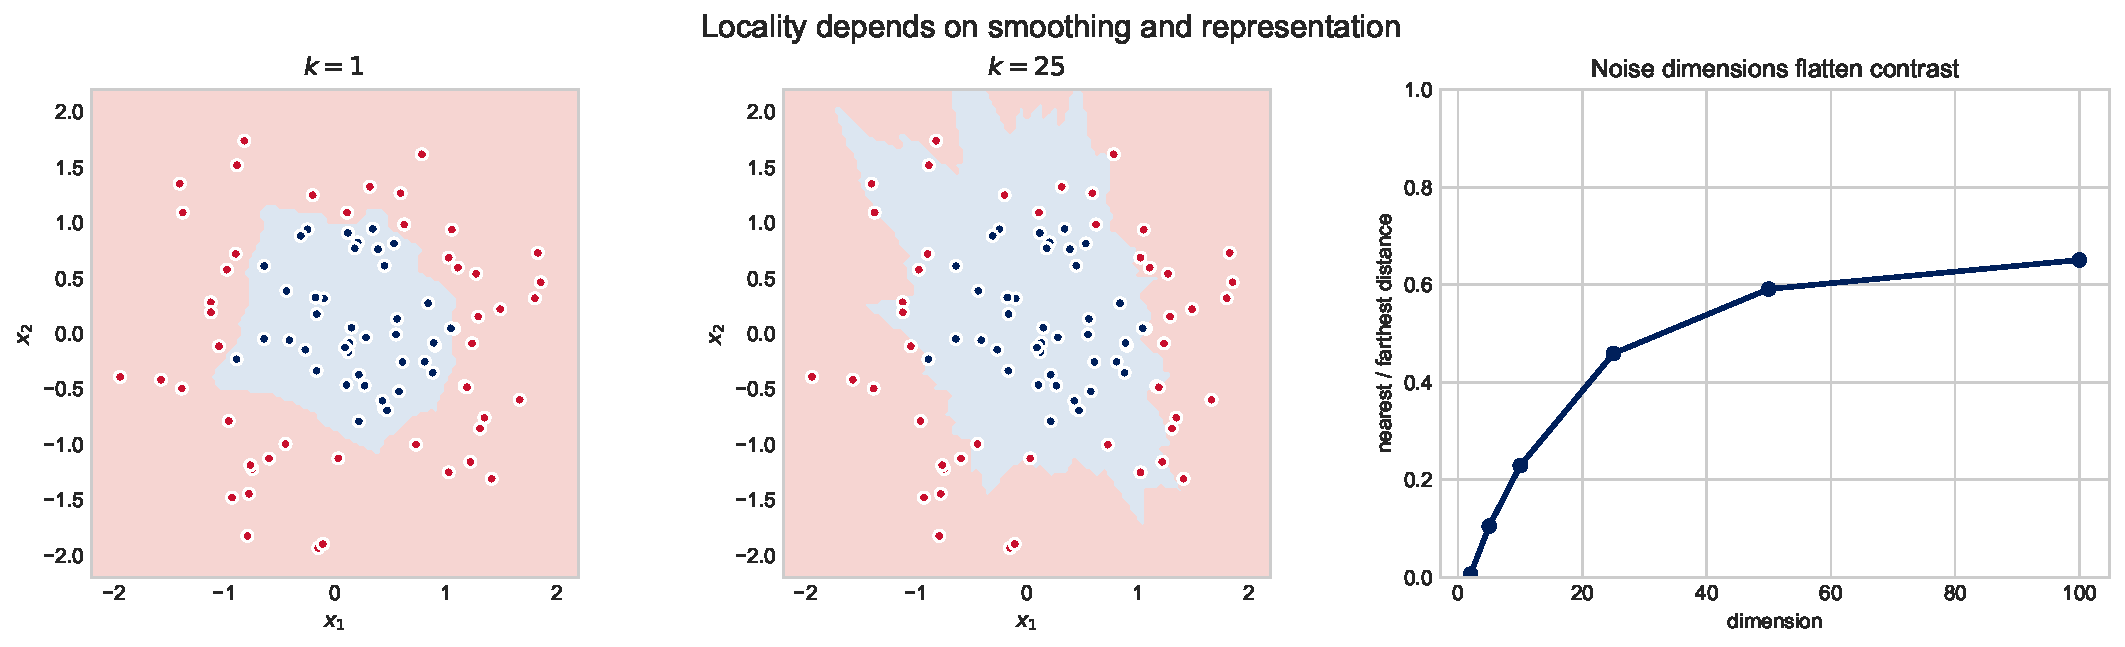
\includegraphics[width=0.98\textwidth]{figures/generated/knn-smoothing-dimensionality.pdf}
  \caption{Left and center: $k$ changes the smoothness of a local classifier.
  Right: independent coordinates reduce nearest-versus-farthest distance
  contrast in one reproducible simulation. The simulation isolates geometry;
  it is not population evidence.}
  \label{fig:knn-smoothing-dimensionality}
\end{figure}

\section{A real classification workflow: wine chemistry}

The Lecture 13 laboratory queries the versioned wine-recognition table. One row
is one Italian wine sample, thirteen features are chemical measurements, and the
target is one of three cultivar classes. Before modeling, the analysis reads the
dataset catalog, verifies identifier uniqueness and missingness, inspects class
counts, and plots scale differences.

The development pipeline compares uniform and inverse-distance votes across a
declared grid of odd $k$ values. Validation accuracy selects a candidate; the
test labels remain hidden. After freezing the configuration, the pipeline refits
the scaler and kNN state on combined development data and reports a
majority-class baseline, held-out accuracy, and a confusion matrix. The
confusion matrix matters because an average can conceal one cultivar's repeated
errors.

This is a complete evaluation contract but a bounded scientific claim. The
sample is small, its collection context limits generalization, and prediction
does not establish that cultivar caused every measured chemical difference.

\section{A real regression workflow: disease progression}

The regression laboratory uses baseline measurements for 442 patients and a
quantitative disease-progression response measured one year later. It chooses
$k$ and weight mode using validation MAE, then reports both MAE and RMSE on the
held-out test data beside a training-mean baseline.

MAE answers the expected absolute target-unit error. RMSE penalizes large errors
more heavily. A residual-versus-prediction plot asks whether errors change over
the response range; inspecting the neighbors of the largest residual asks
whether the query had coherent local support. Feature meanings are incompletely
documented, the sample is small, and no classroom score establishes clinical
utility. The limitation is part of the result.

\begin{misconceptionbox}
\textbf{Misconception:} because kNN is interpretable, a prediction is explained
by listing its neighbors. \textbf{Correction:} neighbor identities reveal the
model's local evidence, but the metric, sampling process, omitted variables,
label quality, and support determine whether those neighbors are meaningful.
An example-based explanation does not validate the underlying similarity.
\end{misconceptionbox}

\section{Recommendation as neighbor retrieval}

A recommender does not merely assign a class. It retrieves and ranks unseen
items from incomplete behavioral evidence. The Lecture 13 laboratory uses an
authentic, deterministic subset of GroupLens MovieLens data: 13,817 rating
events for the 80 most-rated movies in the \code{ml-latest-small} development
dataset. The selection makes class execution reliable but intensifies
popularity bias. It is not a stable research benchmark.

\subsection{Content versus collaborative similarity}

A content-based system compares item attributes such as genres or measured
properties. A collaborative system compares patterns of interaction. Let
$r_{ui}$ be user $u$'s rating of item $i$, and let $\bar r_u$ be that user's
mean observed rating. For users $U_{ij}$ who rated both items $i$ and $j$, an
adjusted cosine similarity is
\[
s(i,j)=
\frac{\sum_{u\in U_{ij}}(r_{ui}-\bar r_u)(r_{uj}-\bar r_u)}
{\sqrt{\sum_{u\in U_{ij}}(r_{ui}-\bar r_u)^2}
 \sqrt{\sum_{u\in U_{ij}}(r_{uj}-\bar r_u)^2}}.
\]
User centering partially separates item preference from generous-versus-strict
rating habits. A minimum co-rating count prevents a single pair of events from
creating apparently perfect similarity.

For user $u$ and unseen item $j$, let $N_k(j;u)$ contain the up-to-$k$ most
positively similar items that the user has rated. A transparent score is
\[
\widehat r_{uj}=\bar r_u+
\frac{\sum_{i\in N_k(j;u)}s(j,i)(r_{ui}-\bar r_u)}
{\sum_{i\in N_k(j;u)}|s(j,i)|}.
\]
The implementation excludes already-seen items and declines candidates with no
positive supported neighbor. Those are testable product rules.

\subsection{Offline evaluation is limited evidence}

A temporal holdout may hide each eligible user's latest positive interaction,
fit on earlier events, and ask whether the hidden item appears in the top-$N$
list. Recall@$N$ or hit rate then measures retrieval of known events. It does
not measure satisfaction for every unseen item because exposure is missing not
at random: an unrated movie may be unknown rather than disliked.

Always compare with a popularity baseline. Also report catalog coverage, list
concentration, novelty or diversity where defensible, and latency. A system can
achieve plausible recall by recommending the same popular items to everyone.
Production evaluation eventually needs user outcomes and guarded experiments,
with explicit protections against feedback loops and harm.

\begin{figure}[htbp]
  \centering
  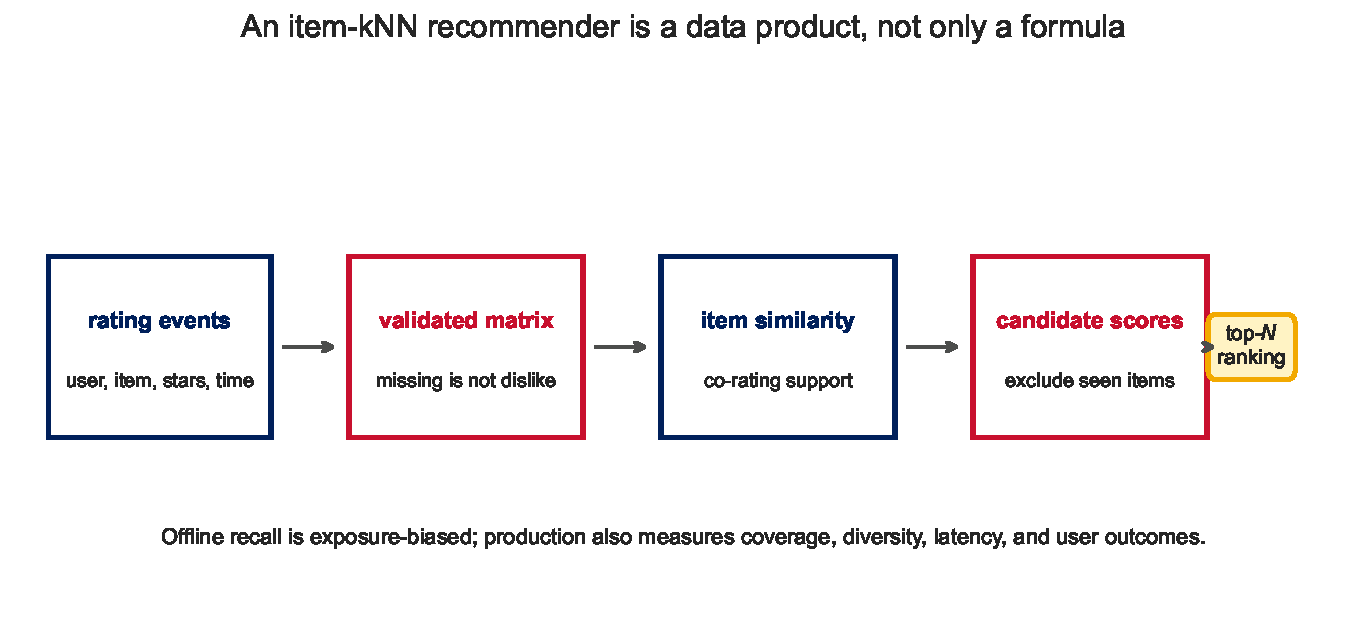
\includegraphics[width=0.98\textwidth]{figures/generated/knn-recommender-system.pdf}
  \caption{Recommendation is an end-to-end data path. Each transition owns a
  contract: event provenance, missingness semantics, similarity support,
  seen-item exclusion, ranking, and operational evaluation.}
  \label{fig:knn-recommender-system}
\end{figure}

\begin{workedexample}{why missing does not mean negative}
Suppose user A rated two science-fiction movies five stars and never rated a
documentary. Encoding the missing documentary rating as zero asserts dislike,
although the user may never have encountered it. A collaborative similarity
calculation therefore operates on co-rated entries and records the overlap
count. A ranking evaluation hides an observed event; it does not manufacture
negative labels from every unobserved pair. This distinction is essential for
both mathematics and data engineering.
\end{workedexample}

\section{Software design: from formula to package}

The course implementation separates three public estimators:
\begin{itemize}
  \item \code{KNearestNeighborsClassifier} stores feature rows and class labels,
  exposes neighbor indices and distances, and predicts normalized vote mass;
  \item \code{KNearestNeighborsRegressor} reuses search while enforcing finite
  numerical responses and local weighted averaging; and
  \item \code{ItemKNNRecommender} validates rating events, builds a sparse-in-meaning
  user-item matrix, fits item similarities, excludes seen items, and ranks
  supported unseen candidates.
\end{itemize}

Hyperparameters are constructor inputs. \code{fit} validates and stores learned
state. \code{predict}, \code{similar\_items}, and \code{recommend} refuse use before fitting.
Input shape, finite-value policy, exact matches, tie ordering, unknown IDs, and
duplicate events have explicit behavior. NumPy-style docstrings and type hints
make the interface reviewable, while exceptions help users locate violated
contracts.

The implementation deliberately uses readable brute-force NumPy. For $n$
training rows and $p$ features, storage is $O(np)$ and one query costs roughly
$O(np)$ before selecting neighbors. A full item-item matrix for $m$ items costs
$O(m^2)$ storage. Larger systems consider sparse operations, tree indexes in
favorable low dimension, or approximate nearest-neighbor methods. Approximation
adds retrieval recall as another evaluated quantity.

\subsection{Tests as executable mathematics}

A serious test suite includes:
\begin{enumerate}
  \item a $3$--$4$--$5$ distance test;
  \item hand-computable class votes and regression means;
  \item properties such as nondecreasing returned distances and probability
  sums;
  \item exact-match behavior under inverse-distance weighting;
  \item invalid $k$, nonfinite input, shape mismatch, and pre-fit use;
  \item differential agreement with a trusted library under matched
  conventions;
  \item recommendation invariants, including no already-seen item; and
  \item clean-kernel execution importing the installed package.
\end{enumerate}
Tests protect public behavior, not private helper names. A useful failure tells
a teammate which mathematical or user-facing contract changed.

\section{The student project handoff}

The companion project template supplies a working production shell. Students
add scientific and product substance without collapsing everything into a
notebook. For a nearest-neighbor contribution, the intended map is
\begin{verbatim}
data/local/your_dataset/                 ignored full or private data
data/fixtures/neighbors/                 small lawful CI fixture
docs/DATASET_CARD.md                     source, license, row meaning, limits
configs/student.toml                     ignored local paths and task config
scripts/fetch_or_validate_your_data.py   reproducible access and validation
src/dsm_project/algorithms/student/neighbors.py
src/dsm_project/algorithms/registry.py   explicit registration
tests/test_student_neighbors.py          executable contracts
notebooks/NN-your-question.ipynb         applied investigation and evidence
\end{verbatim}

``Upload the data'' is not an instruction to commit an arbitrary downloaded
file. License, privacy, size, provenance, and reproducibility determine whether
the repository contains a small fixture, a reviewed database snapshot,
retrieval code plus a checksum, or metadata only. Full local data belongs under
an ignored boundary when redistribution is not justified.

The notebook is named for its question, not merely \code{knn.ipynb}. It imports
student package code, identifies the observation and prediction units, explores
assumptions, compares a baseline, selects on validation evidence, analyzes
failures, and states what can and cannot be concluded. It does not redefine the
estimator, metric, or reusable evaluation function in hidden cells.

\begin{workedexample}{a focused student pull request}
A team investigates whether chemical measurements can retrieve wines with
similar sensory profiles. They first open an issue defining the data license,
observation unit, response, distance, scaling rule, split, baseline, and
latency envelope. On a feature branch they add a validated data adapter, a tiny
public fixture, a NumPy-style documented estimator, analytic and failure tests,
registry entry, and question-led notebook. They run Ruff and pytest locally,
push the branch, and open a pull request that links the issue and interprets
the evidence. Review examines both scientific similarity and software behavior.
Only reviewed package code becomes a candidate for product promotion.
\end{workedexample}

\section{Failure modes and operational evidence}

Common symptoms have diagnostic meaning:
\begin{description}
  \item[Majority predictions everywhere.] $k$ may be too large, class imbalance
  may dominate, or the representation may lack local signal.
  \item[Unit conversion changes results.] Preprocessing is absent or not owned
  by the fitted pipeline.
  \item[Excellent validation, weak deployment.] The split may not reproduce
  time, group, geography, or acquisition shift.
  \item[Fast fit, slow API.] Exact search deferred computation to inference.
  Measure batch size and tail latency.
  \item[Empty recommendation lists.] Co-rating overlap or positive similarity
  is insufficient. Define a safe fallback rather than lowering safeguards
  silently.
  \item[Same recommendations for everyone.] Popularity dominates. Measure
  coverage and concentration beside recall.
\end{description}

A serialized kNN artifact may contain training features, labels, identifiers,
or user histories. Artifact governance must address access, retention,
deletion, encryption, provenance, and retraining. Monitoring can track query
distance, empty-neighborhood rate, latency, feature-schema failures, catalog
coverage, popularity concentration, and delayed outcomes. Logs should identify
model and data versions without exposing sensitive raw records.

\section{Exercises}

\subsection*{Intuition and interpretation}
\begin{enumerate}
  \item Construct two changes of units that reverse the nearest of two points.
  State which units are scientifically defensible.
  \item Explain why a five-of-seven class vote is not necessarily a calibrated
  probability of $5/7$.
  \item Describe a setting where a farthest-neighbor diagnostic is more useful
  than the kNN prediction itself.
  \item Explain why an unrated item is not a negative recommendation label.
\end{enumerate}

\subsection*{Mathematics}
\begin{enumerate}
  \setcounter{enumi}{4}
  \item For query $x=(1,2)$ and training points $(0,0)$, $(2,2)$, $(4,1)$,
  compute Euclidean and Manhattan neighbor orderings.
  \item Derive the inverse-distance regression prediction for targets
  $0$ and $4$ at distances $1.5$ and $0.5$.
  \item Prove that the uniform kNN class vote vector sums to one. State the
  assumption needed about $k$.
  \item In your own words, explain why both $k_n\to\infty$ and $k_n/n\to0$ are
  needed for consistency.
  \item Show that multiplying every coordinate by the same positive constant
  preserves all Euclidean neighbor identities. Give a coordinate-wise scaling
  that does not.
\end{enumerate}

\subsection*{Engineering and contribution}
\begin{enumerate}
  \setcounter{enumi}{9}
  \item Add a test for conflicting labels at zero distance and propose a public
  policy before implementing it.
  \item Benchmark prediction latency for batch sizes $1$, $8$, $64$, and $256$.
  Report median and tail behavior and identify the service implication.
  \item Create a temporal recommender split and compare item kNN with a
  popularity baseline using recall@10 and catalog coverage.
  \item In the project template, open an issue for a domain-aware distance.
  Specify units, invariances, missingness, scaling, analytic tests, and a
  trusted comparison. Implement it only after review of the contract.
  \item Write a dataset-card section explaining whether full data, a CI fixture,
  retrieval code, or metadata may be committed. Support the decision with the
  source terms and privacy boundary.
\end{enumerate}

\begin{chapterreview}
Nearest neighbors turns similarity into a local prediction or retrieval rule.
Classification votes, regression averages, and collaborative recommendation
ranks supported unseen items. The apparent simplicity does not remove modeling
or engineering decisions: representation, metric, scaling, $k$, weighting,
validation, support, dimension, latency, storage, privacy, and update behavior
all belong to the system contract. A professional implementation lives in a
typed package, is protected by analytic and failure tests, is exercised through
real-data notebooks, and enters a product only through reviewed evidence.
\end{chapterreview}

\begin{notebooklink}
Lecture 13 notebook 00 derives neighbor geometry and the package API.
Lecture 13 notebook 01 builds leakage-safe classification and regression pipelines on
real wine-chemistry and diabetes-progression data.
Lecture 13 notebook 02 uses
authentic MovieLens events for collaborative recommendation and maps data,
fixtures, code, tests, notebooks, and pull-request evidence into the companion
student project template.
\end{notebooklink}
